\documentclass[12pt,letterpaper]{article}
\usepackage{listings}
\usepackage{graphicx}
\usepackage[table,xcdraw]{xcolor}
\RequirePackage{xcolor}
\definecolor{tecAzul}{cmyk}{1,0.91,0.33,0.25} % según manual de imagen 2016
\definecolor{tecRojo}{cmyk}{0,0.9,0.86,0}     % según manual de imagen 2016

\renewcommand{\familydefault}{\sfdefault}
\usepackage{amsmath} % for the equation* environment
\usepackage{mwe}
\usepackage{graphicx}
\usepackage[spanish]{babel}
\usepackage{multirow}
\usepackage{titlesec}
\titleformat*{\section}%
{\normalfont\Large\bfseries\color{tecAzul}}
\titleformat*{\subsection}%
{\normalfont\large\bfseries\color{tecAzul}}


\usepackage[tmargin=2cm,bmargin=2cm,lmargin=2.5cm,rmargin=2.5cm]{geometry}
\usepackage{textpos}
\usepackage{tikz}
\usepackage{pgfplots}
\usepackage{pgf}

\usepackage[margin=1cm]{caption}

\usepackage{hyperref}

%
% paragraph layout
%
\parindent0em                           % indentation width of first line
\parskip1.3ex                           % space between paragraphs


\newcommand{\EstudianteA}{David F. Duarte Sánchez}

\pgfplotsset{compat=1.17}



\usepackage{listings}
\usepackage{xcolor}

\definecolor{codegreen}{rgb}{0,0.6,0}
\definecolor{codegray}{rgb}{0.5,0.5,0.5}
\definecolor{codepurple}{rgb}{0.58,0,0.82}
\definecolor{backcolour}{rgb}{0.95,0.95,0.92}

\lstdefinestyle{mystyle}{
    backgroundcolor=\color{backcolour},   
    commentstyle=\color{codegreen},
    keywordstyle=\color{magenta},
    numberstyle=\tiny\color{codegray},
    stringstyle=\color{codepurple},
    basicstyle=\ttfamily\footnotesize,
    breakatwhitespace=false,         
    breaklines=true,                 
    captionpos=b,                    
    keepspaces=true,                 
    numbers=left,                    
    numbersep=5pt,                  
    showspaces=false,                
    showstringspaces=false,
    showtabs=false,                  
    tabsize=2
}

\lstset{style=mystyle}



\begin{document}
	
\graphicspath{{./}{./fig/}}

%-------------------------- Title section -------------------------------------%

%
\begin{textblock}{10}[0,0](-0.5,0)
	\large Escuela de Ingeniería Electrónica \\ 
	EL5617 Trabajo Final de Graduación \\
\end{textblock}

%
\begin{textblock}{10}[0,0](2.6,-0.35)
	\begin{flushright}
		
\includegraphics[scale=0.8]{Firma_TEC-4.pdf}
	\end{flushright}
\end{textblock}

%% Title %%
\begin{center}
	\vspace{70mm}
	{\large\color{tecRojo} Trabajo Final de Graduación}
	\par\vspace{8mm}
	{\Large\bf\color{tecAzul}{Bitácora de Trabajo - Entrega 4}}
	\par\vspace{100mm}
	{{\EstudianteA \\ II Semestre 2024} 
	\vspace{8mm}}
\end{center}

\newpage
%------------------------------------------------------------------------------%

\renewcommand{\baselinestretch}{1.1}    % line spacing

%------------------------------------------------------------------------------%

\section{Semana 8}
\subsection{Corrección de Tesis}

\bf{Fecha de trabajo:} 06/09/2024.\\
\bf{Objetivo:} Corrección de observaciones realizadas a la Tesis.

\begin{table}[h!]
    \resizebox{\textwidth}{!}{%
    \begin{tabular}{|l|}
        \hline
        \hline
        \multicolumn{1}{|c|}{Reporte de   actividades} \\ \hline
        \hline
        -Avances con el sistema embebido, se comienza a probar el sistema operativo a la medida \\
        que se ha elaborado para la tarjeta zedbaord, así como el funcionamiento del mismo primeramente \\
        por medio de un protocolo UART y segundo por medio del protocolo SSH, esto mediante la conexión \\
        de la tarjeta a un router para que la misma se encuentre conectada a la red. \\ \hline
        
        - Se finaliza la elaboración de un manual de usuario, con el fin de hacer más fácil la \\
        evaluación del flujo de trabajo y la depuración del mismo, de esta forma se tendrán\\
        estandarizadas las versiones requeridas y las salidas esperadas en cada uno de los \\
        procedimientos que se realizan a lo largo de la experimentación. \\ \hline
        
        - Se comienza la elaboración de un manual de usuario, con el fin de hacer más fácil la \\
        implementación de capas en el flujo y la depuración del mismo, de esta forma se tendrán\\
        estandarizadas los nombres de carpetas y las jerarquías en cuanto a creación de árboles de dependencias \\
        con el fin de agilizar los procedimientos que se realizan a lo largo de la experimentación. \\ \hline

        - Implementación de una capa de prueba con el objetivo de lograr compilar cualquier archivo en el flujo de trabajo \\
        de yocto, se genera un archivo básico que imprime un hola mundo en consola en yocto, el mismo se debe de ser compilado \\
        por el flujo de trabajo con el fin de optimizar el programa para los recursos de la tarjeta objetivo. \\ \hline

        - Solicitud de una licencia de prueba de matlab embedded coder, con el objetivo de enfocar aun mas el programa generado \\
        al hardware objetivo, Ya que de momento el programa generado por medio del simulink coder genera algunos problemas a la hora \\
        de ser compilado por gcc previo a la compilación generada por yocto \\ \hline\hline
    \end{tabular}}
\end{table}

Se propone el siguiente arbol de dependencias para la capa de prueba generada

\begin{figure}[h!]
    \centering
    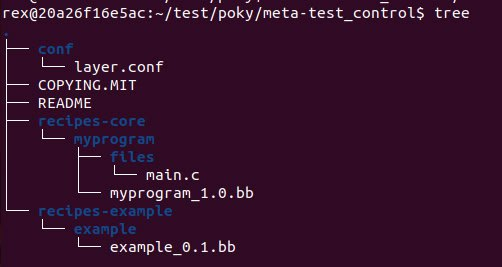
\includegraphics[width=0.8\textwidth]{images/photo_2024-09-19_10-22-43.jpg}
    \caption{Estructura de la receta}
    \label{fig:Entorno}
\end{figure}


\begin{figure}[h!]
    \centering
    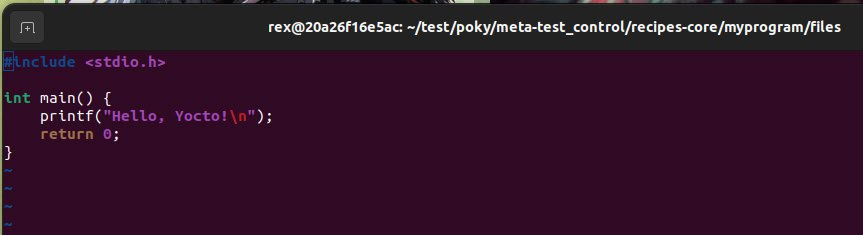
\includegraphics[width=0.8\textwidth]{images/photo_2024-09-19_10-23-44.jpg}
    \caption{Programa de prueba}
    \label{fig:Entorno}
\end{figure}


\begin{figure}[h!]
    \centering
    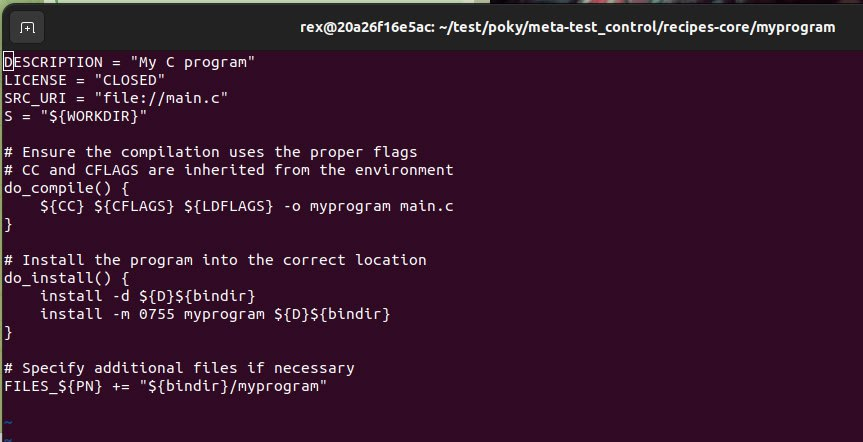
\includegraphics[width=0.8\textwidth]{images/photo_2024-09-19_10-24-37.jpg}
    \caption{Archivo para la compilación del sistema}
    \label{fig:Entorno}
\end{figure}

\begin{figure}[h!]
    \centering
    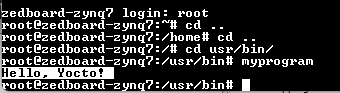
\includegraphics[width=0.8\textwidth]{images/image.png}
    \caption{Sistema implementado en Zedboard}
    \label{fig:Entorno}
\end{figure}


%\bibliography{bibliografia_consultada}
%\bibliographystyle{plain}
\end{document}